\documentclass{article}[18pt]
\ProvidesPackage{format}
%Page setup
\usepackage[utf8]{inputenc}
\usepackage[margin=0.7in]{geometry}
\usepackage{parselines} 
\usepackage[english]{babel}
\usepackage{fancyhdr}
\usepackage{titlesec}
\hyphenpenalty=10000

\pagestyle{fancy}
\fancyhf{}
\rhead{Sam Robbins}
\rfoot{Page \thepage}

%Characters
\usepackage{amsmath}
\usepackage{amssymb}
\usepackage{gensymb}
\newcommand{\R}{\mathbb{R}}

%Diagrams
\usepackage{pgfplots}
\usepackage{graphicx}
\usepackage{tabularx}
\usepackage{relsize}
\pgfplotsset{width=10cm,compat=1.9}
\usepackage{float}

%Length Setting
\titlespacing\section{0pt}{14pt plus 4pt minus 2pt}{0pt plus 2pt minus 2pt}
\newlength\tindent
\setlength{\tindent}{\parindent}
\setlength{\parindent}{0pt}
\renewcommand{\indent}{\hspace*{\tindent}}

%Programming Font
\usepackage{courier}
\usepackage{listings}
\usepackage{pxfonts}

%Lists
\usepackage{enumerate}
\usepackage{enumitem}

% Networks Macro
\usepackage{tikz}


% Commands for files converted using pandoc
\providecommand{\tightlist}{%
	\setlength{\itemsep}{0pt}\setlength{\parskip}{0pt}}
\usepackage{hyperref}

% Get nice commands for floor and ceil
\usepackage{mathtools}
\DeclarePairedDelimiter{\ceil}{\lceil}{\rceil}
\DeclarePairedDelimiter{\floor}{\lfloor}{\rfloor}

% Allow itemize to go up to 20 levels deep (just change the number if you need more you madman)
\usepackage{enumitem}
\setlistdepth{20}
\renewlist{itemize}{itemize}{20}

% initially, use dots for all levels
\setlist[itemize]{label=$\cdot$}

% customize the first 3 levels
\setlist[itemize,1]{label=\textbullet}
\setlist[itemize,2]{label=--}
\setlist[itemize,3]{label=*}

% Definition and Important Stuff
% Important stuff
\usepackage[framemethod=TikZ]{mdframed}

\newcounter{theo}[section]\setcounter{theo}{0}
\renewcommand{\thetheo}{\arabic{section}.\arabic{theo}}
\newenvironment{important}[1][]{%
	\refstepcounter{theo}%
	\ifstrempty{#1}%
	{\mdfsetup{%
			frametitle={%
				\tikz[baseline=(current bounding box.east),outer sep=0pt]
				\node[anchor=east,rectangle,fill=red!50]
				{\strut Important};}}
	}%
	{\mdfsetup{%
			frametitle={%
				\tikz[baseline=(current bounding box.east),outer sep=0pt]
				\node[anchor=east,rectangle,fill=red!50]
				{\strut Important:~#1};}}%
	}%
	\mdfsetup{innertopmargin=10pt,linecolor=red!50,%
		linewidth=2pt,topline=true,%
		frametitleaboveskip=\dimexpr-\ht\strutbox\relax
	}
	\begin{mdframed}[]\relax%
		\centering
		}{\end{mdframed}}



\newcounter{lem}[section]\setcounter{lem}{0}
\renewcommand{\thelem}{\arabic{section}.\arabic{lem}}
\newenvironment{defin}[1][]{%
	\refstepcounter{lem}%
	\ifstrempty{#1}%
	{\mdfsetup{%
			frametitle={%
				\tikz[baseline=(current bounding box.east),outer sep=0pt]
				\node[anchor=east,rectangle,fill=blue!20]
				{\strut Definition};}}
	}%
	{\mdfsetup{%
			frametitle={%
				\tikz[baseline=(current bounding box.east),outer sep=0pt]
				\node[anchor=east,rectangle,fill=blue!20]
				{\strut Definition:~#1};}}%
	}%
	\mdfsetup{innertopmargin=10pt,linecolor=blue!20,%
		linewidth=2pt,topline=true,%
		frametitleaboveskip=\dimexpr-\ht\strutbox\relax
	}
	\begin{mdframed}[]\relax%
		\centering
		}{\end{mdframed}}
\lhead{Networks and Systems - Distributed Systems}


\begin{document}
\begin{center}
\underline{\huge Concurrent events and consistency control}
\end{center}
\section{Concurrency}
\begin{definition}[Shared Object]
May be simultaneously accessed by multiple events (requests into the system)
\end{definition}
\begin{itemize}
	\item A server which manages shared objects is responsible for ensuring the objects remain consistent when accessed by concurrent events
	\item Such a control is called concurrency control
\end{itemize}
Extension to replication - If event T happens before event U in their conflicting access to objects at one of the servers then they must be in that order at all of the servers whose objects are accessed in a conflicting manner by both T and U
\section{Locking}
Grant a lock
\begin{itemize}
	\item Locks on an object are held (in a server) locally
	\item Local lock manager can decide whether to grant a lock or make the requesting transaction wait
\end{itemize}
Issues with Distributed Transmission (DT)
\begin{itemize}
	\item A DT acquires resource located at different servers
	\item Can't release any locks until the transaction has been committed or aborted at all servers involved in the transaction
	\item Objects remain locked and are unavailable for all other transactions during the atomic commit protocol
\end{itemize}
\section{Timestamp ordering}
Timestamp:
\begin{itemize}
	\item Assign a timestamp to each transaction when it starts
	\item Serial equivalence is enforced by committing the versions of objects in the order of the timestamps of transactions that accessed them
	\item Requirement: Globally unique timestamps
\end{itemize}
Distributed Transaction:
\begin{itemize}
	\item The front end is often a good choice to use when setting a global timestamp
	\item Servers of distributed transactions are jointly responsible for ensuring that they are performed in a serially equivalent manner
	\item To achieve the same ordering at all the servers, the coordinators must agree as to the ordering of their timestamps
	\item Issue - In practice, a timestamp is usually assigned by a local server, generating a timestamp, server id pair
\end{itemize}
\section{Concurrent Operations}
In a single machine:
\begin{itemize}
	\item Concurrent operations (events), no matter originated from different or the same machine, are handled by the time sharing feature of an operating system
	\item Operations are implicitly executed one by one in a series under a single clock, i.e. order of operations is well-defined
\end{itemize}
In a distributed system:
\begin{itemize}
	\item Concurrent operations may run on different machines, i.e. distributed transactions
	\item Order of operations can't be easily sorted out due to overlapping operations, clock synchronisation problems, network latency and message loss etc
\end{itemize}
\section{Deadlock Detection}
\begin{itemize}
	\item Local deadlocks can arise within a single server when locking is used for concurrency control
	\item Timeouts: clumsy solution; difficult to choose an appropriate timeout interval, and transactions may be aborted unnecessarily
\end{itemize}
Wait for graph:
\begin{itemize}
	\item Most deadlock detections schemes operate by finding cycles in the transaction wait-for graph
\end{itemize}
\begin{center}
	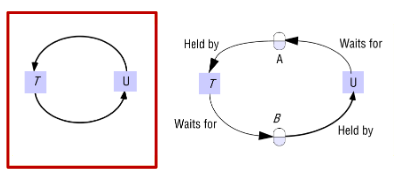
\includegraphics[scale=0.7]{Wait-for}
\end{center}
\subsection{Distributed Deadlock Detection}
\begin{itemize}
	\item Centralised deadlock detection is not a good idea, because it depends on a single server, suffering from poor availability, lack of fault tolerance and no ability to scale
	\item If the global graph is collected less frequently, deadlocks may take longer to be detected
\end{itemize}
Phantom deadlocks
\begin{itemize}
	\item A deadlock that is "detected" but is not really a deadlock
	\item Global deadlock detector requires time to receive local wait-for graphs for constructing the construct the global one. This global wait-for graph may no longer be valid by the time it is constructed
\end{itemize}
Edge chasing:
\begin{itemize}
	\item Don't construct a global wait-for graph
	\item Instead, each server involved attempts to find cycles by forwarding messages called probes
	\item A probe message consists of transaction wait-for relationships representing a (local) path in the global wait for graph
\end{itemize}
\begin{center}
	\includegraphics[scale=0.7]{"Edge Chasing"}
\end{center}
\section{Correctness of replicated objects}
\begin{itemize}
	\item If a system only maintains a single copy for each object, object correctness simply relates to the sequence of operations applied on the object
	\item Correctness of replicated objects is challenging:
	\begin{itemize}
		\item Object copies maintained by different machines, where each machine may receive operations with a different order
	\end{itemize}
	\item Operations are linearisable if:
	\begin{itemize}
		\item The interleaved sequence of operations meets the specification of a (single) correct copy of the objects
		\item The order of operations in the interleaving is consistent with the real times at which the operations occurred in the actual execution
	\end{itemize}
\end{itemize}
\subsection{Linearisability}
There exists a virtual canonical execution - the interleaved operations against a virtual single image of shared (and particularly replicated) objects, and that:
\begin{itemize}
	\item Each client sees a view of the shared objects that is consistent with that single image
	\item i.e. results of the client's operations make sense as they occur within the interleaving
\end{itemize}
\section{Consistency Control}
Issues with distributed systems:
\begin{itemize}
	\item They reply on replicating shared objects, or allowing concurrent access at many nodes
	\item If concurrent accesses of (shared) objects are not carefully controlled, object accesses may be executed in an order different from user expectation, generating incorrect results
\end{itemize}
Modelling of Consistency Control:
\begin{itemize}
	\item Informally, certain object is coherent if the value returned by a read operation is always the value that the user expected
	\item Consistency model: Defined rules for the apparent order and visibility of updates, and it is a continuum with trade-offs
\end{itemize}
\section{Types of consistency}
\begin{definition}[Strict consistency]
	An read on a data item X returned a value corresponding to the result of the most recent write on X
\end{definition}
\begin{definition}[Sequential Consistency]
	If for any transaction there is some interleaving of the series of operations issued by all the clients that satisfies the following two criteria
	\begin{itemize}
		\item The interleaved sequence of operations meets the specification of a (single) correct copy of the contents
		\item The order of operations in the interleaving is consistent with the program order in which each individual process executed them
	\end{itemize}
\end{definition}

\begin{definition}[Casual Consistency]
If event B is caused or influenced by an earlier event A, everyone first see A and then B
\end{definition}




\end{document}